\documentclass[11pt]{amsart}

\usepackage[margin=1.1in]{geometry}
\usepackage{amsmath,amssymb,amsthm,mathtools}
\usepackage{newtxtext,newtxmath}
\usepackage{booktabs,array}
\usepackage{tikz}
\usetikzlibrary{arrows.meta,positioning,fit,backgrounds}
\usepackage[most]{tcolorbox}
\usepackage{enumitem}
\usepackage[hidelinks]{hyperref}
\usepackage{microtype}

\setlength{\parskip}{0.55em plus 0.1em minus 0.05em}
\setlength{\parindent}{0pt}

\allowdisplaybreaks
\setlist[itemize]{topsep=0.35em,itemsep=0.2em,leftmargin=1.8em}
\setlist[enumerate]{topsep=0.35em,itemsep=0.2em,leftmargin=1.8em}

\newtheorem{theorem}{Theorem}[section]
\newtheorem{proposition}[theorem]{Proposition}
\newtheorem{lemma}[theorem]{Lemma}
\newtheorem{corollary}[theorem]{Corollary}
\theoremstyle{definition}
\newtheorem{definition}[theorem]{Definition}
\theoremstyle{remark}
\newtheorem{remark}[theorem]{Remark}

\tcbset{
  keybox/.style={
    enhanced,
    breakable,
    colback=gray!3,
    colframe=gray!35,
    boxrule=0.35pt,
    arc=2pt,
    left=6pt,
    right=6pt,
    top=5pt,
    bottom=5pt,
    before skip=0.8em,
    after skip=0.8em
  },
  theoremstylebox/.style={
    enhanced,
    breakable,
    colback=gray!2,
    colframe=gray!32,
    boxrule=0.3pt,
    arc=2pt,
    left=5pt,
    right=5pt,
    top=5pt,
    bottom=5pt,
    before skip=0.9em,
    after skip=0.9em
  },
  exampleboxstyle/.style={
    enhanced,
    breakable,
    colback=gray!2,
    colframe=gray!28,
    boxrule=0.25pt,
    arc=2pt,
    left=7pt,
    right=7pt,
    top=5pt,
    bottom=5pt,
    before skip=0.8em,
    after skip=0.8em
  }
}

\newtcolorbox{keybox}{keybox}
\newtcolorbox{examplebox}{exampleboxstyle}

\tcolorboxenvironment{definition}{theoremstylebox}
\tcolorboxenvironment{theorem}{theoremstylebox}
\tcolorboxenvironment{proposition}{theoremstylebox}
\tcolorboxenvironment{lemma}{theoremstylebox}
\tcolorboxenvironment{corollary}{theoremstylebox}

\newcommand{\nuu}{\nu_2}
\newcommand{\GD}{G_D}
\newcommand{\CD}{C_D}
\newcommand{\bdD}{\partial_D}
\newcommand{\depth}{\operatorname{depth}}
\newcommand{\dist}{\operatorname{dist}}
\newcommand{\Pre}{\mathsf{Pre}}
\newcommand{\Seed}{\operatorname{Seed}}
\newcommand{\Pair}{\mathsf P}
\newcommand{\Sfam}{\mathcal S}
\newcommand{\eps}{\varepsilon}

\title{A finite graph from the 2-adic valuation of the \texorpdfstring{$3n+1$}{3n+1} map}
\author{Aditya Sriram}

\address{Independent Researcher}
\email{adi.sriram.math@gmail.com}
\date{28 April 2026}

\begin{document}
\begin{abstract}
\setlength{\parskip}{0.55em plus 0.1em minus 0.05em} 
\setlength{\parindent}{0pt} 
This paper builds a finite directed graph $G_D$ from the $2$-adic valuation
data of the $3n+1$ map.

The main result is an explicit bijection for the finite-distance layers of
this adaptive graph.  After quotienting by the top-bit symmetry, the
depth-$d$, distance-$k$ layer is in canonical bijection with
\[
\Sfam_{d,k}
=
\{\Sigma\subseteq[d]:d\in\Sigma,\ |\Sigma|=2k+2\}.
\]
The same history subset also carries the logarithmic drift weight of the
corresponding valuation chain, so the bijection turns the graph into a
usable coordinate system rather than only a counting result.

The paper does not prove a new convergence result for the $3n+1$ problem.
Its contribution is a finite graph-theoretic and enumerative classification
of the adaptive $2$-adic valuation structure that the odd-to-odd map exposes.
\end{abstract}
\maketitle

\section{Introduction}\label{sec:introduction}
The $3n+1$ problem: Given a positive integer $n$, define
\[
T(n)=
\begin{cases}
(3n+1)/2, & n\text{ odd},\\
n/2, & n\text{ even}.
\end{cases}
\]
Pick any positive integer.  Iterate.  The conjecture is that you always
reach~$1$.  We don't know why.  The standard references are Lagarias'
survey~\cite{Lagarias1985} and the annotated bibliographies that
followed~\cite{LagariasAnnotated1999, LagariasAnnotated2009, Lagarias2010}.

Running the map in reverse, every integer has a unique successor, so the predecessors form a tree.
Its branching and stopping-time statistics have been studied extensively~\cite{ApplegateLagarias1995, ApplegateLagarias2003, Wirsching1998}.

A different map can be constructed in the $2$-adic integers.  The odd-to-odd
map
\[
S(x)=\frac{3x+1}{2^{\nu_2(3x+1)}}
\]
extends continuously to $\mathbb{Z}_2$.  Bernstein and Lagarias constructed a
conjugacy map that intertwines the $2$-adic shift with $S$ and analyzed the
induced permutations modulo~$2^n$~\cite{Bernstein1994,
BernsteinLagarias1996}.  The $2$-adic valuation $\nu_2(3x+1)$ is what I study 
in this paper.

In integer space, the predecessor picture is a tree.  In $2$-adic residue
space, it isn't.  A residue class modulo~$2^d$ can have multiple predecessors
at higher depth, and the dynamics between classes can cycle.  Laarhoven and
de~Weger made this precise: at a fixed modulus~$2^d$, the $3n+1$ graph on
residue classes is isomorphic to the binary de~Bruijn graph, and the infinite
$2$-adic limit recovers the Bernstein--Lagarias
conjugacy~\cite{LaarhovenDeWeger2013}.

What happens when a residue class that cannot yet determine its transition is
refined to the next depth instead?  I did not find that question taken up in
the literature.

So I wrote the code and experimented.  At depth~$d$, let a vertex $(r,d)$ represent all odd
integers congruent to $r$ modulo~$2^d$.  Sometimes the class already
determines the next odd-to-odd transition completely, and it gets a forward
edge to a lower-depth class.  Sometimes the visible bits are not enough, and
the class must be split at depth $d+1$.  The result is a finite directed graph
$G_D$ on vertices at varying depths.  It is neither the predecessor tree nor
the fixed-modulus de~Bruijn graph.  It has cycles.

The experiment revealed a graph structure that was surprisingly rigid.  At each 
depth~$d$, exactly $d$ residue classes are \emph{unresolved}: the ones where the visible 
precision does not yet determine the transition.  That count being exactly~$d$ was 
not assumed, it emerged from initial computation and is established in Section~\ref{sec:local}.

The unresolved residues have an explicit algebraic form.  Their
children at depth $d+1$ split one-for-one into a new unresolved residue and a
resolved residue that maps straight to the base class $(1,1)$.  The graph has
a unique nontrivial strongly connected component $C_D$ of
size~$D(D-2)$.

The valuation data turned out to be essential.  The pair of exponents that
determine each edge also carry the $3n+1$ log-drift that appears throughout
the $3n+1$ literature~\cite{Terras1976, Everett1977, Eliahou1993, Tao2022};
the precise connection is worked out in Section~\ref{sec:collatz}.

The concern is that representing an infinite-set problem in a finite structure 
buys you nothing unless the finite object comes with a natural correspondence 
to the data you want to track~\cite{Stanley2012, FlajoletSedgewick2009}.  By 
proving the bijection, structural facts about the adaptive two-adic residue 
dynamics become directly readable from the combinatorics of subsets of~$[d]$.  
For each cutoff~$D$, the graph~$G_D$ has a unique nontrivial strongly connected
component~$C_D$, and every vertex a finite distance outside~$C_D$ carries a 
canonical coordinate built from iterated valuation-preimage pairs.  After the 
natural top-bit quotient, the depth-$d$, distance-$k$ layer is in canonical bijection 
with
\[
\Sfam_{d,k}=\{\Sigma\subseteq[d]:d\in\Sigma,\ |\Sigma|=2k+2\}.
\]
$3n+1$ is the origin of the construction, but what is proved is a finite
graph-theoretic and enumerative statement about adaptive two-adic valuation
data.

\section{The valuation decomposition graph}\label{sec:valuation}\label{sec:graph}
The graph is constructed from one arithmetic operation: the grouped odd-to-odd $3n+1$ step. Everything that follows depends on it. In this section we'll build the intuition first, then dive into definitions.

A vertex is a pair $(r,d)$, where $r$ is an odd residue modulo $2^d$ and $1\le d\le D$.  Think of it as a residue class: all odd integers that look like $r$ when you read their last $d$ binary digits.  The depth $d$ is the amount of precision you have.

The question the graph asks is: \emph{given $d$ bits of precision, can you determine what happens next under the odd-to-odd $3n+1$ map?}

Sometimes you can.  Sometimes you cannot.  That distinction is the whole construction.

\subsection{The decomposition}
Start with a vertex $(r,d)$ and try to carry out the grouped odd-to-odd step~\cite{Wirsching1998}.  Four quantities fall out, in order:

\begin{definition}[Valuation decomposition]\label{def:valuation}
Let $(r,d)$ be a vertex with $r$ odd modulo $2^d$.  Write
\[
t=\nuu(r+1),\qquad q=\frac{r+1}{2^t},\qquad
\rho=\nuu(3^tq-1),\qquad e=d-t-\rho.
\]
The identity $d=e+t+\rho$ is the \emph{valuation decomposition}.

Since \(q\) is odd and \(3^t\) is odd, the product \(3^tq\) is odd. Hence \(3^tq-1\) is even, so \(\rho\ge1\).
\end{definition}



What is each piece doing?

The first quantity, $t$, reads the binary structure of $r+1$.  It counts the trailing zeros: how many times you divide by $2$ before hitting an odd number.  The quotient $q=(r+1)/2^t$ is that odd number.

The second quantity, $\rho$, reads the binary structure of $3^tq-1$.  After multiplying the odd quotient by $3^t$ and subtracting $1$, you again count trailing zeros.

Together, $t$ and $\rho$ consume precision.  You started with $d$ bits.  Reading $t$ costs $t$ of them; reading $\rho$ costs $\rho$ more.  What remains is
\[
e=d-t-\rho.
\]
That is the \emph{output precision}: the number of bits still available to identify the next residue class.

If $e\ge1$, there is enough precision left.  The transition is determined.  If $e<1$, the visible bits have been entirely consumed and the transition is ambiguous.

That's the entirety of the underlying mechanism. The following examples show it in action.

\subsection{Four examples}\label{subsec:examples}

\begin{table}[htbp]
\centering
\renewcommand{\arraystretch}{1.15}
\begin{tabular}{cccccl}
\toprule
$(r,d)$ & $t$ & $q$ & $\rho$ & $e$ & outcome \\
\midrule
$(1,4)$ & $1$ & $1$ & $1$ & $2$ & resolved $\to(1,2)$ \\
$(5,4)$ & $1$ & $3$ & $3$ & $0$ & unresolved \\
$(5,5)$ & $1$ & $3$ & $3$ & $1$ & resolved $\to(1,1)$ \\
$(21,5)$ & $1$ & $11$ & $5$ & $-1$ & unresolved \\
\bottomrule
\end{tabular}
\smallskip
\caption{The valuation decomposition at four vertices.  Rows~3 and~4 are the two children of the unresolved vertex in row~2.}
\label{tab:examples}
\end{table}

Row~1 is the baseline.  At $(1,4)$, the precision budget is $d=4$.  Reading $t$ costs $1$ bit; reading $\rho$ costs $1$ more; two bits survive.  That is enough output precision to identify a target class, so the vertex is resolved: $(1,4)\to(1,2)$.

Row~2 is the contrast.  At $(5,4)$, the budget is still $d=4$, but now $\rho=3$.  After $t$ takes its bit, $\rho$ swallows everything that remains.  The output precision is $e=0$.  The vertex is unresolved: four bits were not enough.

Rows~3 and~4 show what happens next.  The unresolved vertex $(5,4)$ splits into two children at depth~$5$: the residues $(5,5)$ and $(21,5)$.  Both inherit $t=1$ from the same trailing-zero structure, but the extra bit of depth changes their fates.  For $(5,5)$, $\rho$ stays at~$3$ and the new bit survives as $e=1$: the vertex resolves to $(1,1)$.  For $(21,5)$, $\rho$ grows to~$5$ and devours the new bit along with it, leaving $e=-1$: the vertex remains unresolved.

One child resolved; the other did not.  That asymmetry is not an accident. It is the structural mechanism that drives the entire graph.  Section~\ref{sec:local} proves that it holds in general: every non-maximal unresolved vertex, upon refinement, produces exactly one resolved child and one unresolved child.

\subsection{Resolved and unresolved vertices}

The examples illustrate the two cases that define the graph.

When $e\ge1$, the vertex is \emph{resolved}.  The decomposition determines a unique target $(s,e)$, where $s$ is the odd residue of $\frac{3^tq-1}{2^\rho}$ modulo $2^e$.  The graph records this as a directed edge:
\[
(r,d)\to(s,e).
\]
Each such edge carries a weight that measures logarithmic drift defined in Section~\ref{sec:weighted}.

When $e<1$, the vertex is \emph{unresolved}.  The $d$ visible bits were not enough.  In the graph, the unresolved vertex has no valuation edge.  Instead, the class splits into two refined vertices at depth $d+1$:
\[
(r,d)\;\longmapsto\;(r,\,d+1),\quad (r+2^d,\,d+1).
\]
These two children see one additional bit.  One of them may now resolve; the other may need further refinement.  The pattern of how this splitting propagates is the subject of Section~\ref{sec:local}.

\subsection{The graph $G_D$}

The finite directed graph $G_D$, for a positive integer cutoff $D$, is now fully specified:
\begin{itemize}
\item \textbf{Vertices}: all pairs $(r,d)$ with $1\le d\le D$ and $r$ odd modulo $2^d$.
\item \textbf{Valuation edges}: each resolved vertex $(r,d)$ has a single outgoing edge to its target $(s,e)$.
\item \textbf{Refinement}: each unresolved vertex at depth $d<D$ splits into two children at depth $d+1$.  At depth $D$, unresolved vertices have no outgoing edges.
\end{itemize}

The graph is neither the predecessor tree of the integers nor the de~Bruijn graph at a fixed modulus.  It is an adaptive structure: resolved vertices move to lower depth; unresolved vertices move to higher depth.  The interplay between these two directions is what gives $G_D$ its rigid internal structure.

\begin{figure}[htbp]
\centering
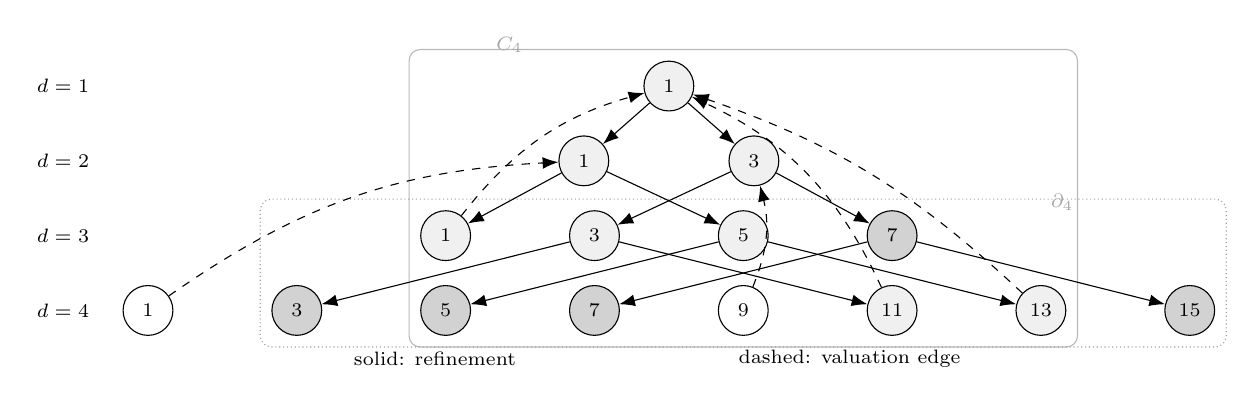
\begin{tikzpicture}[
  x=1.35cm,
  y=0.95cm,
  vertex/.style={circle,draw,inner sep=1.2pt,minimum size=18pt,font=\scriptsize},
  core/.style={vertex,fill=gray!12},
  boundary/.style={vertex,fill=gray!35},
  outside/.style={vertex,fill=white},
  redge/.style={-{Latex[length=2mm]},thin},
  vedge/.style={-{Latex[length=2mm]},thin,dashed},
  comp/.style={draw,rounded corners,gray!55,inner sep=4pt},
  bdy/.style={draw,rounded corners,gray!75,densely dotted,inner sep=4pt}
]

% depth 1
\node[core] (v11) at (0,0) {$1$};

% depth 2
\node[core] (v12) at (-0.8,-1) {$1$};
\node[core] (v32) at (0.8,-1) {$3$};

% depth 3
\node[core] (v13) at (-2.1,-2) {$1$};
\node[core] (v33) at (-0.7,-2) {$3$};
\node[core] (v53) at (0.7,-2) {$5$};
\node[boundary] (v73) at (2.1,-2) {$7$};

% depth 4
\node[outside] (v14) at (-4.9,-3) {$1$};
\node[boundary] (v34) at (-3.5,-3) {$3$};
\node[boundary] (v54) at (-2.1,-3) {$5$};
\node[boundary] (v74) at (-0.7,-3) {$7$};
\node[outside] (v94) at (0.7,-3) {$9$};
\node[core] (v114) at (2.1,-3) {$11$};
\node[core] (v134) at (3.5,-3) {$13$};
\node[boundary] (v154) at (4.9,-3) {$15$};

% refinement edges
\draw[redge] (v11) -- (v12);
\draw[redge] (v11) -- (v32);
\draw[redge] (v12) -- (v13);
\draw[redge] (v12) -- (v53);
\draw[redge] (v32) -- (v33);
\draw[redge] (v32) -- (v73);
\draw[redge] (v33) -- (v34);
\draw[redge] (v33) -- (v114);
\draw[redge] (v53) -- (v54);
\draw[redge] (v53) -- (v134);
\draw[redge] (v73) -- (v74);
\draw[redge] (v73) -- (v154);

% valuation edges
\draw[vedge,bend left=18] (v13) to (v11);
\draw[vedge,bend left=16] (v14) to (v12);
\draw[vedge,bend right=18] (v94) to (v32);
\draw[vedge,bend right=20] (v114) to (v11);
\draw[vedge,bend right=12] (v134) to (v11);

\begin{scope}[on background layer]
\node[comp,fit=(v11)(v12)(v32)(v13)(v33)(v53)(v114)(v134)] (cfit) {};
\node[bdy,fit=(v73)(v34)(v54)(v74)(v154)] (bfit) {};
\end{scope}

\node[font=\scriptsize] at (-5.7,0) {$d=1$};
\node[font=\scriptsize] at (-5.7,-1) {$d=2$};
\node[font=\scriptsize] at (-5.7,-2) {$d=3$};
\node[font=\scriptsize] at (-5.7,-3) {$d=4$};
\node[font=\scriptsize,gray!70] at (-1.5,0.55) {$C_4$};
\node[font=\scriptsize,gray!70] at (3.7,-1.55) {$\partial_4$};
\node[font=\scriptsize] at (-2.2,-3.65) {solid: refinement};
\node[font=\scriptsize] at (1.7,-3.65) {dashed: valuation edge};
\end{tikzpicture}
\caption{The adaptive graph $G_4$.  The label inside a vertex is the odd residue $r$ at the displayed depth.  The shaded rounded region is the unique nontrivial strongly connected component $C_4$; the dotted rounded region is the boundary $\partial_4$.}
\label{fig:G4}
\end{figure}

\section{Local structure}\label{sec:local}
In this section I explore why the unresolved vertex $(5,4)$ split into two children at depth~$5$, one of which resolved and one of which did not. This section proves that the pattern is not an accident.  It holds for every non-maximal unresolved vertex, and it is the mechanism behind everything that follows.

The first task is to identify the unresolved residues explicitly.

The condition $e\le0$ means $3^tq\equiv1\pmod{2^{d-t}}$: the
remaining $d-t$ bits of precision are exactly absorbed, and there is
nothing left to read $\rho$ from.  Since $r+1=2^tq$, this forces
\[
r_{d,t}\equiv 2^t(3^t)^{-1}-1\pmod{2^d},
\qquad 1\le t<d.
\]
For each value of $t$ between $1$ and $d-1$, there is exactly one such residue.  Set $r_{d,d}=2^d-1$, the residue whose binary expansion is all ones.  These $d$ residues are the \emph{unresolved residues} at depth~$d$, and they are distinct since
$\nuu(r_{d,t}+1)=t$.  Every other odd residue modulo $2^d$ is \emph{resolved}.

That the count is exactly~$d$ is worth pausing on.  It was not built into the construction; it fell out of the constraint $e\le0$.  At depth~$d$, you have $d$ bits of precision, and exactly $d$ residue classes consume all of them.

An unresolved residue of type $t<d$ is \emph{non-maximal}; the
remaining case $r_{d,d}=2^d-1$ is \emph{maximal}.  The maximal vertex is distinguished: it is the only unresolved residue where $t=d$, meaning the trailing-zero count of $r+1$ equals the full depth.  Its refinement behavior, as the lemma below shows, differs from the rest.

\begin{lemma}[Direct returns]\label{lem:directreturns}
Every non-maximal unresolved vertex, when refined, produces one child
that stays unresolved and one resolved child that maps to $(1,1)$.
The maximal vertex produces two unresolved children.
Call the resolved child a \emph{direct return}.  At depth $d$ there are
exactly $\max(d-2,0)$ direct returns.
\end{lemma}

\begin{proof}
For the non-maximal case, the two depth-$(d+1)$ lifts of
$(r_{d,t},d)$ replace $q$ by $q$ and $q+2^{d-t}$.  Since
\[
3^t(q+2^{d-t})-1=(3^tq-1)+3^t\cdot 2^{d-t},
\]
exactly one satisfies the stronger congruence modulo $2^{d+1-t}$;
that is the unresolved child of type~$t$.  The other has $\rho=d-t$,
giving target depth~$1$.

For the maximal case, the two children of $(2^d-1,d)$ are $2^d-1$ and
$2^{d+1}-1$: the unresolved residues of types $d$ and $d+1$ at
depth $d+1$.  Neither is a direct return.

The non-maximal unresolved vertices at depth $d-1$ are those of types
$1,\ldots,d-2$, each contributing one direct return at depth~$d$.
The count is $\max(d-2,0)$.
\end{proof}

This asymmetry is crucial. Every non-maximal unresolved vertex, upon one step of refinement, sends one child back to $(1,1)$ and keeps the other unresolved for the next depth. As the splitting propagates to higher depth, the same one-for-one pattern repeats.

\section{The unique nontrivial SCC}\label{sec:core}

The splitting from Section~\ref{sec:local} creates cycles. Unresolved vertices refine to direct returns, and direct returns map back to $(1,1)$. The question is whether those cycles all belong to a single component, and what lies outside it.

In this section I show that $G_D$ has one nontrivial strongly connected component. Every vertex either belongs to it, flows into it, or is trapped on the boundary.

First, the boundary.  Lemma~\ref{lem:directreturns} guarantees that every unresolved vertex produces at least one unresolved child at the next depth.  At depth~$D$, there is no next depth.  All $D$ unresolved vertices at depth~$D$ — types $1,\ldots,D-1$ together with the maximal type~$D$ — have no outgoing valuation edges and no room to refine; call them \emph{terminal}.  The maximal unresolved vertex at depth $D-1$, namely $(2^{D-1}-1,D-1)$, refines only into terminal vertices.  Together these $D+1$ vertices form the boundary~$\bdD$.  Nothing leaves it.

\begin{theorem}[SCC theorem]\label{thm:core}
For $D\ge3$, $G_D$ has a unique nontrivial strongly connected
component $C_D$.  It consists of all unresolved vertices and direct
returns outside the boundary, and
\[
|C_D|=D(D-2).
\]
A vertex reaches $C_D$ if and only if it is not in $\bdD$.
\end{theorem}

For $D=1$ and $D=2$, the graph is degenerate: the boundary appears before any direct-return cycle can form, so there is no nontrivial strongly connected component.  The theorem therefore begins at the first nondegenerate cutoff, $D=3$.

\begin{proof}
The argument has four parts: the claimed set is strongly connected,
everything outside it flows in, no other cycle exists, and the count is $D(D-2)$.

\emph{Strong connectivity.}
Every direct return maps to $(1,1)$.  Every non-maximal unresolved
vertex in $C_D$ has a direct-return child
(Lemma~\ref{lem:directreturns}), and hence a path to $(1,1)$.  Every
maximal unresolved vertex in $C_D$ has depth at most $D-2$, since it
is not on the boundary; one refinement step produces a non-maximal
unresolved child, and the previous case applies. Conversely, every unresolved residue 
at depth \(d\) reduces modulo \(2^{d-1}\) to an unresolved residue at depth \(d-1\). 
Indeed, for
\(t<d\),
\[
r_{d,t}\equiv 2^t(3^t)^{-1}-1 \pmod{2^d}
\]
reduces to the same defining congruence at depth \(d-1\), with the
case \(t=d\) reducing to the maximal residue \(2^{d-1}-1\).  Thus each
unresolved vertex has an unresolved parent, and induction gives a
refinement path from \((1,1)\) to it.  Every direct return is a
refinement child of an unresolved vertex, so \((1,1)\) reaches all of
\(C_D\).

\emph{Absorption.}
Let $v$ be a resolved vertex that is not a direct return.  It has a valuation edge, since the alternative $e\le0$ would make it unresolved.  That edge lands at depth $e=d-t-\rho$, which is at most $d-2$ because $t\ge1$ and $\rho\ge1$.  In particular, no valuation edge from depth at most~$D$ can reach depth $D-1$ or~$D$.  Since the boundary sits entirely at those depths, iterating valuation edges reaches $C_D$ before the boundary.

\emph{No other cycles.}
Outside \(C_D\), an unresolved vertex is a boundary vertex and has no
outgoing refinement edge.  A resolved vertex outside \(C_D\) has a
valuation edge; if that edge does not enter \(C_D\), then its target
has depth \(e=d-t-\rho<d\).  Thus any path outside \(C_D\) either
terminates at the boundary or follows valuation edges of strictly
decreasing depth.  Neither behavior permits a cycle.

\emph{Count.}
The unresolved vertices across depths $1$ through $D$ number
\[
\sum_{d=1}^{D}d=\frac{D(D+1)}{2}.
\]
The direct returns across depths $3$ through $D$ number
\[
\sum_{d=3}^{D}(d-2)=\frac{(D-1)(D-2)}{2}.
\]
Their union has size $D^2-D+1$.  The boundary removes $D$ terminal unresolved vertices at depth~$D$ and the maximal vertex $(2^{D-1}-1,D-1)$ at depth $D-1$, for a total of $D+1$.  Thus
\[
|C_D|=D^2-D+1-(D+1)=D(D-2).
\]
\end{proof}

\section{Preimages and pair indexing}\label{sec:preimages}
With $C_D$ now defined, this section focuses on the resolved vertices outside $C_D$. The previous section showed that such a vertex eventually reaches $C_D$, but what information determines that inward step?

To answer this question, I look at the edges from the other direction. Fix a target vertex and find all sources whose valuation edge points to it.

I find that a preimage is not determined by an arbitrary residue at some higher depth. Rather, it is determined by exactly two intermediate depths: the depth $i=e+t$ at which the trailing-zero count~$t$ is read, and the source depth $j=e+t+\rho$ at which~$\rho$ is read.  Those two numbers pin down the source residue completely.

\begin{theorem}[Preimage-pair theorem]\label{thm:preimage}
Fix a target vertex $(s,e)\in V(\GD)$.  The valuation-edge preimages
of $(s,e)$ are canonically indexed by pairs
\[
e<i<j\le D.
\]
For the pair $(i,j)$, set
\[
t=i-e,
\qquad
\rho=j-i,
\qquad
d=j.
\]
Then the unique source is the pair $(r,j)$, where \(r\) is the odd residue
of \(2^tq-1\) modulo \(2^j\), and \(q\) is the unique odd solution to
\[
q\equiv 3^{-t}(1+2^\rho s)\pmod {2^{e+\rho}}.
\]
Write
\[
\Pre_{i,j}(s,e)=(r,j)
\]
for this source.  Consequently the number of valuation-edge preimages
of \((s,e)\) is
\[
\binom{D-e}{2}.
\]
\end{theorem}

\begin{proof}
By the valuation decomposition, a source of depth \(d\) with target depth
\(e\) satisfies
\[
d=e+t+\rho.
\]
Thus
\[
i=e+t,
\qquad
j=d
\]
satisfy \(e<i<j\le D\).

Conversely, fix \(e<i<j\le D\) and put
\[
t=i-e,
\qquad
\rho=j-i.
\]
A source with target residue \(s\) must satisfy
\[
3^tq-1\equiv 2^\rho s \pmod {2^{e+\rho}},
\]
or equivalently
\[
q\equiv 3^{-t}(1+2^\rho s)\pmod {2^{e+\rho}}.
\]
Since \(3\) is a unit modulo any power of \(2\), the inverse \(3^{-t}\)
exists.  Hence this congruence has a unique solution modulo
\(2^{e+\rho}\), and that solution is odd.

Let \(r\) be the odd residue of \(2^tq-1\) modulo \(2^j\).  Then
\[
r+1\equiv 2^tq \pmod {2^j},
\]
with \(q\) odd, so \(\nuu(r+1)=t\).

It remains to check that the second valuation is exactly \(\rho\).  The
congruence
\[
3^tq-1\equiv 2^\rho s \pmod {2^{e+\rho}}
\]
gives
\[
3^tq-1=2^\rho(s+2^e m)
\]
for some integer \(m\).  Since \(s\) is odd and \(e\ge1\), the factor
\(s+2^e m\) is odd.  Therefore
\[
\nuu(3^tq-1)=\rho
\]
exactly.  Dividing by \(2^\rho\) gives target residue \(s\) modulo
\(2^e\).  Thus \((r,j)\) is a valuation-edge preimage of \((s,e)\).

Uniqueness follows from the same congruence for \(q\).  Once the pair
\((i,j)\) is fixed, the values of \(t\), \(\rho\), and \(j\) are fixed,
and the congruence determines \(q\) modulo \(2^{e+\rho}\).  Therefore it
determines the odd residue \(r\) modulo \(2^j\).

Finally, the indexing pairs are exactly the two-element subsets of
\(\{e+1,\ldots,D\}\).  Hence the number of valuation-edge preimages of
\((s,e)\) is
\[
\binom{D-e}{2}.
\]
\end{proof}

The pair attached to a valuation edge $v=(r,d)\to(s,e)$ is therefore
\[
\Pair(v)=\{e+\nuu(r+1),\,d\}.
\]
The first element marks the depth at which $t$ was read. The second marks the source depth, which is where $\rho$ was determined.  Each preimage step inserts exactly two new depths between the target depth and the source depth.  When preimage steps are composed into chains — a vertex at distance $k$ from $C_D$ passing through $k$ successive targets — the inserted pairs interleave without collision.

\section{Histories as coordinates}\label{sec:histories}
With $C_D$ preimage pairs as context, this section can now answer:
Given a vertex outside $C_D$, what does its valuation chain produce?

The answer, as it turns out, is a subset of $[d]$.  It is built from two ingredients: a
label for the endpoint in $C_D$, and a record of the preimage pairs
traversed along the chain.  I split the work across two sections.  This
section assembles the coordinate, and the next one shows that it is
complete.

\begin{examplebox}
\textbf{Running example.}
Fix $D=7$ and the vertex $v=(43,7)$.  Its valuation chain is
\[
  (43,7)\xrightarrow{\;e_2\;}(1,4)\xrightarrow{\;e_1\;}(1,2)\in C_D,
\]
so $R_D(v)=2$.  This chain will serve as the illustration for the concepts, definitions, and proofs 
that follow.
\end{examplebox}

\textbf{Let}
\[
R_D(v)=
\begin{cases}
\operatorname{dist}(v,C_D), & \text{if } v \text{ reaches } C_D,\\
\infty, & \text{otherwise.}
\end{cases}
\]

\begin{keybox}
If $R_D(v)=k>0$, then $v$ is resolved and not a direct return, and
repeated valuation edges give a unique chain
\[
v=v_k\to v_{k-1}\to\cdots\to v_0\in C_D.
\]
\end{keybox}

For our example, $k=2$, $v_2=(43,7)$, $v_1=(1,4)$, and $v_0=(1,2)$.

For $d\ge2$, let $\tau_d$ be the top-bit involution
\[
\tau_d(r,d)=
\begin{cases}
(r+2^{d-1},d),&r<2^{d-1},\\
(r-2^{d-1},d),&r>2^{d-1}.
\end{cases}
\]
It exchanges the two depth-$d$ lifts of the same residue modulo~$2^{d-1}$.
The quotient is such that the subset coordinate will ignore this
top bit, while the sign coordinate will remember it.

\begin{examplebox}
\textit{Example (Involution at depth~2).}
The endpoint of our chain is $v_0=(1,2)$.  Its partner under $\tau_2$ is
$(1+2^1,2)=(3,2)$.  One checks that $(3,2)$ is the terminal vertex of the
parallel chain starting at $(43+2^6,7)=(107,7)$: both chains pass through
the same sequence of residue classes modulo $2^{d-1}$, differing only in
their top bits at every step.
\end{examplebox}

\begin{proposition}[Seed orbits away from the boundary]\label{prop:seeds}
For $2\le d\le D-2$, the quotient $(C_D\cap V_d)/\tau_d$ is
canonically labeled by the two-element sets
\[
\{a,d\},\qquad 1\le a<d.
\]
There are two oriented vertices of $C_D$ above each label.
\end{proposition}

\begin{proof}
For $1\le a\le d-2$, the two children of the unresolved vertex of
type $a$ at depth $d-1$ consist of the unresolved vertex of type $a$
at depth $d$ and its direct-return sibling.  These two children differ
by $2^{d-1}$, so they form one $\tau_d$-orbit.  The remaining orbit
comes from the two children of the maximal unresolved vertex at depth
$d-1$, namely the unresolved vertices of types $d-1$ and $d$.  Since
$d\le D-2$, no boundary vertex is involved.  These $d-1$ two-element
orbits exhaust $C_D\cap V_d$.
\end{proof}

\begin{definition}[Seed and orientation]\label{def:orientation}
Let $v_0=(r,d)\in C_D$ with $2\le d\le D-2$.  

Define
\(
\Seed(v_0)=\{a,d\}
\)
to be the label of its $\tau_d$-orbit from Proposition~\ref{prop:seeds}.

Its orientation is the top-bit sign
\[
\eps(v_0)=
\begin{cases}
-,&1\le r<2^{d-1},\\
+,&2^{d-1}<r<2^d.
\end{cases}
\]

For any positive-distance vertex $v$, define $\eps(v)$ to be the
orientation of the terminal vertex $v_0\in C_D$ in its valuation
chain.
\end{definition}

\textit{Example (Seed and orientation of $v_0=(1,2)$).}
The endpoint of our running chain is $(1,2)$.  It lies in the unique
$\tau_2$-orbit at depth~$2$, so
\[
  \Seed(1,2)=\{1,2\}.
\]
Since $r=1<2^1=2$, the orientation is $\eps=-$.  The top-bit partner
$(3,2)$ has the same seed but $r=3>2$, giving $\eps=+$.  The two
$\tau_2$-partners carry opposite signs and the same seed label.

\subsection{The history set}\label{subsec:general-history}

The second ingredient records the chain itself.  Each edge
$v_m\to v_{m-1}$ contributes a preimage pair
$\{d_{m-1}+t_m,\,d_m\}$ from Section~\ref{sec:preimages}.
Collecting the seed and all preimage pairs into a single set gives the
history.

If $v=v_k\to\cdots\to v_0\in C_D$ is the unique chain for a vertex
of positive finite distance, write $v_m=(r_m,d_m)$. The endpoint $v_0$ lies away
from the truncation boundary:
\[
2\le d_0\le D-2,
\]
because the final edge is not a direct return and every valuation edge
lowers depth by at least two. 

\begin{keybox}
Define the projected history
\[
\Sigma(v)=\Seed(v_0)\cup\bigcup_{m=1}^k\{d_{m-1}+\nuu(r_m+1),d_m\}.
\]
\end{keybox}

For a stable vertex of $C_D$ itself, set $\Sigma(v_0)=\Seed(v_0)$.

The seed contributes two elements.  Each of the $k$ preimage steps
contributes two more.  The following lemma says these contributions
never collide.

\begin{lemma}[History intervals]\label{lem:historyintervals}
If $v$ has finite distance $k$ and depth $d$, then the union defining
$\Sigma(v)$ is disjoint.  For $k\ge1$,
\[
\Sigma(v)\subseteq[d],\qquad d\in\Sigma(v),\qquad |\Sigma(v)|=2k+2.
\]
\end{lemma}

\begin{proof}
For the edge $v_m\to v_{m-1}$, write $t_m$ and $\rho_m$ for the
decomposition data.  Then
\[
d_m=d_{m-1}+t_m+\rho_m,
\]
so
\[
\{d_{m-1}+t_m,d_m\}\subset(d_{m-1},d_m].
\]
The seed lies in $[1,d_0]$.  Inducting along the chain, each preimage
step appends two new elements in the next interval $(d_{m-1},d_m]$.
Hence the union is disjoint, lies in $[d]$, contains the final
depth~$d$, and has cardinality $2+2k$.
\end{proof}

\textit{In our example.}
The chain has $k=2$ steps.  The three contributions live in
non-overlapping intervals:
\begin{align*}
  \Seed(1,2)=\{1,2\}&\subset[1,2]=(d_0\text{-seed}),\\
  \text{pair for }e_1=\{3,4\}&\subset(2,4]=(d_0,d_1],\\
  \text{pair for }e_2=\{6,7\}&\subset(4,7]=(d_1,d_2].
\end{align*}
These intervals are pairwise disjoint, confirming disjointness of
$\Sigma(43,7)=\{1,2,3,4,6,7\}$.  The cardinality is $2+2\cdot2=6$, the
depth $7$ is the largest element, and the whole set is contained in $7$.

\subsection{The running example in full}\label{subsec:full-example}
Table~\ref{tab:history-ex} collects the complete computation for the
chain $(43,7)\to(1,4)\to(1,2)$, showing how each piece of the
coordinate is assembled.

\begin{table}[htbp]
\centering
\renewcommand{\arraystretch}{1.15}
\begin{tabular}{clccccl}
\toprule
step & vertex & $t$ & $\rho$ & $e$ & pair & interval\\
\midrule
seed & $(1,2)\in C_D$ & --- & --- & --- & $\{1,2\}$ & $[1,2]$\\
$e_1$ & $(1,4)$ & $1$ & $1$ & $2$ & $\{3,4\}$ & $(2,4]$\\
$e_2$ & $(43,7)$ & $2$ & $1$ & $4$ & $\{6,7\}$ & $(4,7]$\\
\bottomrule
\end{tabular}
\smallskip
\caption{Seed and preimage pairs for the chain
  $(43,7)\to(1,4)\to(1,2)$.  The three contributions occupy
  non-overlapping intervals, so their union is automatically disjoint.}
\label{tab:history-ex}
\end{table}

Collecting seed and pairs:
\[
\Sigma(43,7)=\{1,2\}\cup\{3,4\}\cup\{6,7\}=\{1,2,3,4,6,7\}.
\]
Six elements ($2k+2=6$), contained in $[7]$, with $7\in\Sigma$.
The orientation is $\eps=-$ (since $r_0=1<2^1=2$).  The full
coordinate of $(43,7)$ is
\[
  (\eps,\Sigma)=\bigl(-,\;\{1,2,3,4,6,7\}\bigr).
\]
The gap at position~$5$ reflects that the second edge had trailing-zero 
count $t=2$ rather than~$t=1$, so the lower element of the pair $\{6,7\}$ skipped~$5$.

For contrast, the vertex $(45,7)$ follows the same intermediate
targets but has $t=1$, $\rho=2$ at the second step.  Its preimage
pair is $\{5,7\}$ instead of $\{6,7\}$, giving
\[
\Sigma(45,7)=\{1,2,3,4,5,7\}.
\]
Same cardinality, same endpoints, different subset.  The gap moved
from position~$5$ to position~$6$.  Different chains produce
different histories.

\begin{keybox}
For a positive-distance vertex \(v\), the full coordinate is
\(
(\eps(v),\Sigma(v)).
\)
\end{keybox}

\section{Reconstruction and binomial layers}\label{sec:bijection}
In this section, by reversing the process, we show that every admissible subset
reconstructs exactly one chain, the coordinate is a bijection, and the
layer counts are binomial coefficients.

\begin{examplebox}
\textbf{Running example.}
We continue with $D=7$, $v=(43,7)$, and the coordinate computed in
Section~\ref{sec:histories}:
\(
  (\eps,\Sigma)=\bigl(-,\;\{1,2,3,4,6,7\}\bigr),\qquad k=2,\quad d=7.
\)
\end{examplebox}

\begin{definition}[Admissible history subsets]\label{def:Sfam}
A distance-$k$ history has two seed entries and two entries from each
of its \(k\) preimage steps, so it has \(2k+2\) entries in total.  For
\(k\ge1\), define
\[
\Sfam_{d,k}
=
\{\Sigma\subseteq[d]:d\in\Sigma,\ |\Sigma|=2k+2\}.
\]
Elements of \(\Sfam_{d,k}\) are called admissible history subsets.
\end{definition}

\begin{examplebox}
\textit{Example ($\Sfam_{7,2}$).}
With $d=7$ and $k=2$, the family $\Sfam_{7,2}$ consists of all
$6$-element subsets of $[7]$ that contain $7$.  There are
$\binom{6}{5}=6$ such subsets, and our coordinate has
$\Sigma=\{1,2,3,4,6,7\}\in\Sfam_{7,2}$, confirming that the history
map lands in the right family.
\end{examplebox}

\begin{theorem}[History bijection]\label{thm:bijection}
For $D\ge3$, $k\ge1$, and $1\le d\le D$, the map
\[
v\longmapsto (\eps(v),\Sigma(v))
\]
is a canonical bijection
\[
\{v:\depth(v)=d,\ R_D(v)=k\}
\longrightarrow
\{+,-\}\times\Sfam_{d,k}.
\]
Here canonical means that the inverse is computed by the explicit
preimage construction of Theorem~\ref{thm:preimage}.  Consequently
\[
\bigl|\{v:\depth(v)=d,\ R_D(v)=k\}\bigr|=2\binom{d-1}{2k+1}.
\]
\end{theorem}

For $D=1$ and $D=2$, there are no positive finite-distance layers outside a nontrivial $C_D$.  Thus the statement is vacuous in the degenerate cases excluded above.

\begin{proof}
Lemma~\ref{lem:historyintervals} shows that the map lands in
$\{+,-\}\times\Sfam_{d,k}$.
To reconstruct, take $(\eps,\Sigma)$ with
\[
\Sigma=\{\sigma_1<\sigma_2<\cdots<\sigma_{2k+2}=d\}.
\]
Start with the oriented vertex of $C_D$ labeled by
$\{\sigma_1,\sigma_2\}$ and orientation $\eps$.  At step
$m=1,\ldots,k$, use Theorem~\ref{thm:preimage} to take the unique
valuation-edge preimage of the current target of depth $\sigma_{2m}$
indexed by the pair
\[
\sigma_{2m}<\sigma_{2m+1}<\sigma_{2m+2}.
\]
This constructs a chain whose final source has depth $d$.
Each reconstructed edge has target depth at least $2$, so no
reconstructed source is a direct return; hence the first time the
chain reaches $C_D$ is its prescribed endpoint.  Thus the final source
has distance $k$.  The construction is inverse to the history map
because Theorem~\ref{thm:preimage} gives a unique source for each
target and pair.
\end{proof}

\subsection{Reconstruction by example}\hfill \break
\textbf{Given.}\enspace $\eps=-$, $\Sigma=\{1,2,3,4,6,7\}$,
Write $\Sigma=\{\sigma_1,\ldots,\sigma_6\}=\{1<2<3<4<6<7\}$.

\textbf{Step 0 (seed).}\enspace
$\Seed=\{\sigma_1,\sigma_2\}=\{1,2\}$, orientation $\eps=-$.

The vertex of $C_D$ with seed $\{1,2\}$ and orientation $-$ is
$(1,2)$: the unresolved vertex of type~$1$ at depth~$2$, which
satisfies $1<2^1$.  Set $v_0=(1,2)$.

\textbf{Step 1.}\enspace Preimage pair
$(\sigma_3,\sigma_4)=(3,4)$.

Target: $v_0=(1,2)$ at depth $e=2$.  The pair satisfies $2<3<4$.
Apply Theorem~\ref{thm:preimage}: $t=3-2=1$, $\rho=4-3=1$, source
depth $d=4$.  The unique source is $(1,4)$.  Set $v_1=(1,4)$.

\textbf{Step 2.}\enspace Preimage pair
$(\sigma_5,\sigma_6)=(6,7)$.

Target: $v_1=(1,4)$ at depth $e=4$.  The pair satisfies $4<6<7$.
Apply Theorem~\ref{thm:preimage}: $t=6-4=2$, $\rho=7-6=1$, source
depth $d=7$.  The unique source is $(43,7)$.  Set $v_2=(43,7)$.

The output is $v=(43,7)$ at distance $k=2$.  The subset was consumed
two elements at a time, left to right.  Each step required nothing
beyond the pair and the current target.

\subsection{Top-bit equivariance}\label{subsec:topbit}

The bijection splits every distance layer into two copies indexed by
$\eps\in\{+,-\}$.  That doubling is a top-bit artifact: the
involution $\tau_d$ commutes with the entire valuation chain, so
quotienting by it removes the orientation cleanly.

\begin{lemma}[Top-bit equivariance]\label{lem:topbit}
Let $v=(r,d)$ be a resolved vertex with valuation edge to $(s,e)$,
and suppose $e\ge2$.  Then $\tau_d(v)$ is resolved with the same
values of $t$ and $\rho$, and its valuation edge lands at
$\tau_e(s,e)$.
\end{lemma}

\begin{proof}
Apply the valuation decomposition to $v$: $t=\nuu(r+1)$,
$q=(r+1)/2^t$, $\rho=\nuu(3^tq-1)$, and $d=e+t+\rho$.  Replacing
$r$ by its top-bit flip changes $r+1$ to
\[
r+1\pm2^{d-1}.
\]
Since $e\ge2$ and $\rho\ge1$, one has $d-1>t$, so the value of $t$
is unchanged.  The corresponding odd quotient is
\[
q'=q\pm2^{d-1-t}.
\]
Then
\[
3^tq'-1=(3^tq-1)\pm3^t2^{d-1-t}.
\]
The added term has two-adic valuation $d-1-t=\rho+e-1>\rho$, so the
exact value of $\rho$ is also unchanged.  After division by $2^\rho$,
the target odd representative changes by
\[
\pm 3^t2^{e-1},
\]
which is congruent modulo $2^e$ to adding or subtracting the top bit
$2^{e-1}$.  Hence the target is $\tau_e(s,e)$.
\end{proof}

\textit{In our example.}
The chain
\(
(43,7)\to(1,4)\to(1,2)
\)
is carried by the top-bit involution to
\(
(107,7)\to(9,4)\to(3,2).
\)
The values of $t$ and $\rho$ are unchanged at both steps, so the two
chains have the same history subset
\(
\Sigma=\{1,2,3,4,6,7\}
\)
and opposite orientations. Flipping the top bit flips the orientation and nothing else.

\begin{corollary}[Quotient layers]\label{cor:quotient}
For $k\ge1$ and $d\ge2$,
\[
\{v:\depth(v)=d,\ R_D(v)=k\}/\tau_d
\cong
\Sfam_{d,k}.
\]
Equivalently, summing over $d\le D$,
\[
\bigl|\{v:R_D(v)=k\}\bigr|=2\binom{D}{2k+2}.
\]
\end{corollary}

\begin{proof}
Positive-distance valuation chains never use a direct-return edge, and
every target depth along such a chain is at least $2$.
Lemma~\ref{lem:topbit} therefore shows that the whole chain commutes
with the top-bit involution.  The involution changes only the
orientation coordinate $\eps$ and leaves the subset history $\Sigma$
unchanged.  Quotienting Theorem~\ref{thm:bijection} by this
two-element orientation gives the first claim.

For the total count, sum the oriented layer count:
\[
\sum_{d=1}^D2\binom{d-1}{2k+1}
=
2\sum_{d=2k+2}^D\binom{d-1}{2k+1}
=
2\binom{D}{2k+2},
\]
where the last equality is the hockey-stick identity.
\end{proof}

\textit{In our example.}
Take $D=7$, $k=2$.  The formula predicts
\[
\bigl|\{v:R_7(v)=2\}\bigr|=2\binom{7}{6}=14.
\]
Summing the oriented layer counts confirms this:
\[
\sum_{d=6}^{7}2\binom{d-1}{5}
=2\binom{5}{5}+2\binom{6}{5}
=2\cdot1+2\cdot6=14.
\]
The vertex $(43,7)$ and its partner $(107,7)$ form one
$\tau_7$-orbit in the quotient family $\Sfam_{7,2}$.

\section{Weighted histories}\label{sec:weighted}
The history coordinate also records the additive statistic that corresponds to $3n+1$ logarithmic drift: the quantity that measures, along a chain of odd-to-odd steps, whether the iterates are collectively growing or shrinking.  That statistic runs through the entire $3n+1$ literature, from Terras's stopping-time analysis~\cite{Terras1976} to Tao's density theorem~\cite{Tao2022}.  In this section, let's consider $G_D$ as a weighted directed graph by assigning a real weight to each valuation edge, and show that the total weight along a chain factors through the subset history.

Put
\[
\alpha=\log_2 3.
\]
If $v=(r,d)$ is resolved with valuation edge to $(s,e)$, the valuation decomposition gives $d=e+t+\rho$.  Define the edge weight
\[
\omega(v)=t\alpha-(t+\rho)=t\alpha-(d-e).
\]
The term $t\alpha$ accounts for $t$ multiplications by~$3$; the term $t+\rho$ accounts for $t+\rho$ divisions by~$2$.  Their difference is the net logarithmic drift of the step.  Section~\ref{sec:collatz} derives this from the $3n+1$ map directly.

Equivalently, if the pair of the edge is
\[
\Pair(v)=\{i,j\},\qquad e<i<j=d,
\]
then
\[
\omega(v)=(i-e)\alpha-(j-e).
\]

Now let $v$ have positive finite distance $R_D(v)=k$, and write its valuation chain as
\[
v=v_k\to v_{k-1}\to\cdots\to v_0\in C_D.
\]
The total chain weight is
\[
\Omega(v)=\sum_{m=1}^k \omega(v_m).
\]
The endpoint vertex in $C_D$ carries no weight in this definition; only the valuation edges in the distance chain are counted.

The claim is that this total weight depends only on the subset history $\Sigma(v)$, with no residue data needed.  To state this precisely, I define a weight directly on subsets.

For a history
\[
\Sigma=\{\sigma_1<\sigma_2<\cdots<\sigma_{2k+2}=d\}\in\Sfam_{d,k},
\]
define the alternating-gap sum
\[
\Lambda(\Sigma)=\sum_{m=1}^k(\sigma_{2m+1}-\sigma_{2m})
\]
and the history weight
\[
\Omega(\Sigma)=\Lambda(\Sigma)\alpha-(d-\sigma_2).
\]
I use the same letter $\Omega$ for both because the theorem below identifies the two.

\subsection{Example: weight from the subset alone}\label{subsec:weight-ex}

The claim that the total weight depends only on~$\Sigma$ is concrete enough to verify by hand.  The two distance-$2$ vertices from the example above share the same chain of targets. Both pass through $(1,4)$ and land at $(1,2)$, but differ in their second preimage step.

\begin{table}[htbp]
\centering
\small
\renewcommand{\arraystretch}{1.15}
\begin{tabular}{ccccccc}
\toprule
vertex & $\Sigma$ & edge & $t$ & $\rho$ & $\omega$ & $\Omega$\\
\midrule
$(43,7)$ & $\{1,2,3,4,6,7\}$
  & $(1,4)\to(1,2)$ & $1$ & $1$ & $\alpha-2$ & \\
  & & $(43,7)\to(1,4)$ & $2$ & $1$ & $2\alpha-3$ & $3\alpha-5$\\[4pt]
$(45,7)$ & $\{1,2,3,4,5,7\}$
  & $(1,4)\to(1,2)$ & $1$ & $1$ & $\alpha-2$ & \\
  & & $(45,7)\to(1,4)$ & $1$ & $2$ & $\alpha-3$ & $2\alpha-5$\\
\bottomrule
\end{tabular}
\smallskip
\caption{Two vertices at the same depth and distance, sharing the same intermediate target $(1,4)$ and the same endpoint $(1,2)$, but with different histories and different total weights.}
\label{tab:weight-ex}
\end{table}

Now compute the history weight directly from the subsets.

For $\Sigma=\{1,2,3,4,6,7\}$: the odd-indexed gaps after the seed are $\sigma_3-\sigma_2=3-2=1$ and $\sigma_5-\sigma_4=6-4=2$, so $\Lambda=3$ and $\Omega=3\alpha-(7-2)=3\alpha-5$.

For $\Sigma=\{1,2,3,4,5,7\}$: the odd-indexed gaps are $\sigma_3-\sigma_2=3-2=1$ and $\sigma_5-\sigma_4=5-4=1$, so $\Lambda=2$ and $\Omega=2\alpha-(7-2)=2\alpha-5$.

Both match.  The residue data, $43$ versus $45$, the odd quotients, the intermediate representatives, have dropped out.  The weight sees only the gaps between elements of~$\Sigma$.

\begin{theorem}[Weight factorization through histories]\label{thm:weightfactor}
Let $D\ge3$, $k\ge1$, and let $v$ be a vertex with $R_D(v)=k$ and $\depth(v)=d$.  Then
\[
\Omega(v)=\Omega(\Sigma(v)).
\]
Consequently the total chain weight depends only on the quotient history $\Sigma(v)$ and is independent of the orientation $\eps(v)$.
\end{theorem}

\begin{proof}
Write the distance chain as
\[
v=v_k\to v_{k-1}\to\cdots\to v_0\in C_D,
\]
and put $v_m=(r_m,d_m)$.  For each edge $v_m\to v_{m-1}$, write $t_m$ and $\rho_m$ for the decomposition data.  By the definition of the history coordinate, if
\[
\Sigma(v)=\{\sigma_1<\sigma_2<\cdots<\sigma_{2k+2}=d\},
\]
then the $m$th valuation preimage step has
\[
d_{m-1}=\sigma_{2m},\qquad d_{m-1}+t_m=\sigma_{2m+1},\qquad d_m=\sigma_{2m+2}.
\]
Therefore
\[
t_m=\sigma_{2m+1}-\sigma_{2m},
\qquad
 t_m+\rho_m=d_m-d_{m-1}=\sigma_{2m+2}-\sigma_{2m}.
\]
Summing the edge weights gives
\begin{align*}
\Omega(v)
&=\sum_{m=1}^k\bigl(t_m\alpha-(t_m+\rho_m)\bigr)\\
&=\alpha\sum_{m=1}^k(\sigma_{2m+1}-\sigma_{2m})
  -\sum_{m=1}^k(\sigma_{2m+2}-\sigma_{2m})\\
&=\Lambda(\Sigma(v))\alpha-(\sigma_{2k+2}-\sigma_2)\\
&=\Lambda(\Sigma(v))\alpha-(d-\sigma_2).
\end{align*}
This is exactly $\Omega(\Sigma(v))$.  Since $\Sigma(v)$ is unchanged by switching the top-bit orientation, the total chain weight is independent of $\eps(v)$.
\end{proof}

The proof is a telescoping calculation, but the conclusion is not obvious from the definitions.  The residue data — the actual values $r_m$ and the odd quotients $q_m$ at each step — have dropped out completely.  The total log-drift sees only the gaps between elements of the subset $\Sigma$.

\begin{corollary}[Weighted quotient layers]\label{cor:weightedquotient}
For $k\ge1$ and $d\ge2$, the quotient bijection
\[
\{v:\depth(v)=d,\ R_D(v)=k\}/\tau_d\cong\Sfam_{d,k}
\]
is weight-preserving when the left side is weighted by total chain weight and $\Sfam_{d,k}$ is weighted by $\Omega(\Sigma)$.
\end{corollary}

\begin{remark}
The statistic $\Lambda(\Sigma)$ selects the odd-numbered gaps after the seed depth $\sigma_2$, while $d-\sigma_2$ is the total depth gained after the seed.  Thus the weight is an alternating-gap functional on the same subsets that index the binomial distance layers:
\[
\Omega(\Sigma)
=
\alpha\bigl[(\sigma_3-\sigma_2)+(\sigma_5-\sigma_4)+\cdots+(\sigma_{2k+1}-\sigma_{2k})\bigr]
-(d-\sigma_2).
\]
This is the structural point of the weighted theorem: once the seed is fixed, the log-drift sees only the odd-indexed inserted gaps and the total post-seed depth gain.  No information from the orientation coordinate is needed.
\end{remark}

Section~\ref{sec:collatz} explains where the edge weight comes from and what it measures: the residue-class part of the $3n+1$ multiplicative drift, derived directly from the odd-to-odd $3n+1$ map.

\section{Origin of the rule and meaning of the weight}\label{sec:collatz}

The rule used to define $G_D$ is extracted from a residue-class model of the odd $3n+1$ dynamics.  In that model one studies the odd-to-odd valuation update
\[
X+1=2^tq,
\qquad
3^tq-1=2^\rho Y.
\]
This is not the usual one-step map $X\mapsto (3X+1)/2^{\nuu(3X+1)}$.  Rather, it is a grouped valuation step: the first equation records a run-length $t$ determined by the binary position of $X+1$, and the second equation records the power of two removed after multiplying the odd quotient by $3^t$.

The adaptive graph keeps exactly the residue-class information needed to know this grouped step.  If a depth-$d$ class determines $t$ and determines $\rho$ before the visible precision is exhausted, it has a valuation edge.  If the visible precision is exhausted, the class is unresolved and must be refined.  This is why unresolved vertices refine and resolved vertices move to lower depth.

The same equations explain the edge weight.  Since
\[
Y=\frac{3^tX+3^t-2^t}{2^{t+\rho}},
\]
one has
\[
\log_2(Y/X)
=
t\log_2 3-(t+\rho)
+
\log_2\!\left(1+\frac{1-(2/3)^t}{X}\right).
\]
For large lifts $X$ in a fixed residue class, the last term is $O(1/X)$.  Thus the graph weight
\[
\omega=t\log_2 3-(t+\rho)
\]
is precisely the residue-class part of the $3n+1$ multiplicative drift.  Along a finite chain, $\Omega(v)$ is the sum of these local log-drift terms.  Theorem~\ref{thm:weightfactor} says that this finite residue-level drift is a function only of the subset history $\Sigma$.

This connects the paper to the standard logarithmic bookkeeping used throughout $3n+1$ analysis.  In cycle and stopping-time arguments, one compares the accumulated power of $3$ with the accumulated power of $2$; in logarithmic form this is a sum of terms of the shape
\[
(\text{number of }3\text{-multiplications})\log_2 3
-
(\text{number of }2\text{-divisions}).
\]
The present paper does not add a convergence claim to that tradition.  Its contribution is to show that, for the finite adaptive valuation graph, the corresponding log-functional has an exact combinatorial coordinate: the binomial subset history.

The statements proved here therefore have a deliberately limited scope.  A vertex $(r,d)$ is a residue class, not an integer.  The integer $1$ is represented by an infinite compatible tower of residue classes, and integer dynamics require lift data beyond any fixed $G_D$.  What the graph supplies is a finite, classifiable object: adaptive two-adic refinement produces a unique nontrivial SCC, pair-indexed valuation preimages, a top-bit symmetry, binomial distance layers, and a history-level log-drift functional.

\section*{Disclosure}\label{sec:disclosure}
The author used ChatGPT 5.4 and ChatGPT 5.5 for editorial assistance with LaTeX formatting, spellcheck, and grammar. The mathematical content, including the definitions, proofs, code, and conclusions are the author's own.

\begin{thebibliography}{99}

\bibitem{ApplegateLagarias1995}
D. Applegate and J. C. Lagarias.
The distribution of $3x+1$ trees.
\emph{Experimental Mathematics} 4 (1995), no.~3, 193--209.

\bibitem{ApplegateLagarias2003}
D. Applegate and J. C. Lagarias.
Lower bounds for the total stopping time of $3x+1$ iterates.
\emph{Mathematics of Computation} 72 (2003), no.~242, 1035--1049.

\bibitem{Bernstein1994}
D. J. Bernstein.
A non-iterative $2$-adic statement of the $3n+1$ conjecture.
\emph{Proceedings of the American Mathematical Society} 121 (1994), no.~2, 405--408.

\bibitem{BernsteinLagarias1996}
D. J. Bernstein and J. C. Lagarias.
The $3x+1$ conjugacy map.
\emph{Canadian Journal of Mathematics} 48 (1996), no.~6, 1154--1169.

\bibitem{Eliahou1993}
S. Eliahou.
The $3x+1$ problem: new lower bounds on nontrivial cycle lengths.
\emph{Discrete Mathematics} 118 (1993), no.~1--3, 45--56.

\bibitem{Everett1977}
C. J. Everett.
Iteration of the number-theoretic function $f(2n)=n$, $f(2n+1)=3n+2$.
\emph{Advances in Mathematics} 25 (1977), no.~1, 42--45.

\bibitem{FlajoletSedgewick2009}
P. Flajolet and R. Sedgewick.
\emph{Analytic Combinatorics}.
Cambridge University Press, 2009.

\bibitem{Lagarias1985}
J. C. Lagarias.
The $3x+1$ problem and its generalizations.
\emph{The American Mathematical Monthly} 92 (1985), no.~1, 3--23.

\bibitem{LagariasAnnotated1999}
J. C. Lagarias.
The $3x+1$ problem: an annotated bibliography (1963--1999).
Preprint, arXiv:math/0309224, 2003.

\bibitem{LagariasAnnotated2009}
J. C. Lagarias.
The $3x+1$ problem: an annotated bibliography, II (2000--2009).
Preprint, arXiv:math/0608208, 2006.

\bibitem{Lagarias2010}
J. C. Lagarias, editor.
\emph{The Ultimate Challenge: The $3x+1$ Problem}.
American Mathematical Society, Providence, RI, 2010.

\bibitem{LaarhovenDeWeger2013}
T. Laarhoven and B. de Weger.
The Collatz conjecture and de Bruijn graphs.
\emph{Indagationes Mathematicae} 24 (2013), no.~4, 971--983.

\bibitem{Stanley2012}
R. P. Stanley.
\emph{Enumerative Combinatorics, Volume 1}.
Cambridge Studies in Advanced Mathematics 49, 2nd ed., Cambridge University Press, 2012.

\bibitem{Tao2022}
T. Tao.
Almost all orbits of the Collatz map attain almost bounded values.
\emph{Forum of Mathematics, Pi} 10 (2022), e12.

\bibitem{Terras1976}
R. Terras.
A stopping time problem on the positive integers.
\emph{Acta Arithmetica} 30 (1976), 241--252.

\bibitem{Wirsching1998}
G. J. Wirsching.
\emph{The Dynamical System Generated by the $3n+1$ Function}.
Lecture Notes in Mathematics 1681, Springer, 1998.

\end{thebibliography}
\end{document}
